\section{Classification}

Classification problems involve predicting a qualitative (categorical) response variable \(Y\) based on one or more predictor variables \(X\).  

\subsection{Quantitative vs. Qualitative Outcomes}

\begin{itemize}
    \item \textbf{Quantitative outcomes:} \(Y \in \mathbb{R}\). Typically modeled with regression, minimizing a loss function such as least squares.
    \item \textbf{Qualitative outcomes:} \(Y \in \{1, 2, \dots, K\}\). These are modeled using classification methods like logistic regression or generative models.
\end{itemize}

\subsection{Feature Vector and Notation}

Let 
\[
\mathbf{X} = (X_1, X_2, \dots, X_p)^T
\] 
be the feature vector. For example, in the \textbf{IRIS dataset}, the features are:
\[
X_1 = \text{Sepal Length}, \quad X_2 = \text{Sepal Width}, \quad X_3 = \text{Petal Length}, \quad X_4 = \text{Petal Width}
\] 
and the response \(Y \in \{\text{setosa, versicolor, virginica}\}\).

The predicted class is:
\[
g(\mathbf{x}) = \arg\max_{k} P(Y = k \mid \mathbf{X} = \mathbf{x})
\]

\subsection{Logistic Regression (Binary Case)}

The probability of class 1 is modeled as:
\[
P(Y=1 \mid X=x) = \frac{e^{\beta_0 + \beta_1 x}}{1 + e^{\beta_0 + \beta_1 x}}
\]

The log-odds (logit) transformation gives a linear relationship:
\[
\log \frac{P(x)}{1 - P(x)} = \beta_0 + \beta_1 x
\]

\[
\begin{cases} 
\beta_1 > 0 & \text{increasing $x$ increases $P(x)$} \\
\beta_1 < 0 & \text{increasing $x$ decreases $P(x)$} 
\end{cases}
\]

\subsection{Maximum Likelihood Estimation (MLE)}

The likelihood function is:
\[
L(\beta_0, \beta_1) = \prod_{i=1}^{n} P(x_i)^{y_i} \left[ 1 - P(x_i) \right]^{1 - y_i}
\]

MLE maximizes the likelihood (or equivalently, minimizes the negative log-likelihood):
\[
\hat{\beta}_0, \hat{\beta}_1 = \arg\max_{\beta_0, \beta_1} L(\beta_0, \beta_1)
\]

\subsection{Multinomial Logistic Regression}

For \(K>2\) classes, probabilities are modeled using the \textbf{softmax function}:
\[
P(Y=k \mid X=x) = \frac{e^{\beta_{k0} + \beta_k^T x}}{\sum_{j=1}^{K} e^{\beta_{j0} + \beta_j^T x}}
\]

The log-odds relative to a baseline class \(K\) are:
\[
\log \frac{P(Y=k \mid X=x)}{P(Y=K \mid X=x)} = \beta_{k0} + \beta_k^T x
\]

\subsection{Generative Models}

Generative models estimate:
\[
P(X \mid Y=k) \quad \text{and} \quad P(Y=k)
\] 
Then, using Bayes' theorem:
\[
P(Y=k \mid X=x) = \frac{P(X=x \mid Y=k) P(Y=k)}{\sum_{j=1}^K P(X=x \mid Y=j) P(Y=j)}
\]

\subsection{Additive Models and Least Squares}

For continuous responses:
\[
Y = f_\theta(X) + \epsilon, \quad \epsilon \sim N(0, \sigma^2)
\]

MLE reduces to minimizing the sum of squared errors (RSS):
\[
\hat{\theta} = \arg\min_\theta \sum_i \left( Y_i - f_\theta(X_i) \right)^2
\]

\subsection{Visualizing Logistic Regression Decision Boundary}

\begin{tikzpicture}[scale=1.0]
\draw[->] (0,0) -- (6,0) node[right] {$X$};
\draw[->] (0,0) -- (0,4) node[above] {$P(Y=1|X)$};
\draw[domain=0:5, smooth, variable=\x, blue, thick] plot ({\x}, {4/(1+exp(-1*(\x-2)))});
\draw[dashed] (2,0) -- (2,2) -- (0,2);
\node at (3.5,3.5) {Sigmoid curve};
\node at (2.5,0.3) {$x_0$};
\end{tikzpicture}

\subsection{Generative Models and Advanced Classification}

Generative models estimate the joint distribution \(P(X,Y)\) and then use Bayes' theorem to compute class probabilities:
\[
P(Y=k \mid X=x) = \frac{P(Y=k) P(X=x \mid Y=k)}{P(X=x)}
\]

Here:
\begin{itemize}
    \item \(P(Y=k)\) is the prior probability of class \(k\)
    \item \(P(X=x \mid Y=k)\) is the class-conditional density
    \item \(P(X=x) = \sum_{i=1}^K P(Y=i) P(X=x \mid Y=i)\) by the law of total probability
\end{itemize}

\subsubsection{Linear Discriminant Analysis (LDA)}

LDA assumes that:
\begin{itemize}
    \item Each class \(k\) has a Gaussian distribution with mean \(\mu_k\) and a **common covariance matrix** \(\Sigma\)
    \item The decision boundary is linear in \(x\)
\end{itemize}

The discriminant function is:
\[
\delta_k(x) = x^T \Sigma^{-1} \mu_k - \frac{1}{2} \mu_k^T \Sigma^{-1} \mu_k + \log \pi_k
\]
where \(\pi_k\) is the prior probability of class \(k\).  

The predicted class is:
\[
\hat{y} = \arg\max_k \delta_k(x)
\]

We estimate unknown parameters from the data:
\[
\hat{\mu}_k = \frac{1}{n_k} \sum_{i: y_i=k} x_i, \quad
\hat{\Sigma} = \frac{1}{n-K} \sum_{k=1}^K \sum_{i: y_i=k} (x_i - \hat{\mu}_k)(x_i - \hat{\mu}_k)^T
\]

\subsubsection*{Decision Boundary Visualization (2 Classes, 2 Features)}
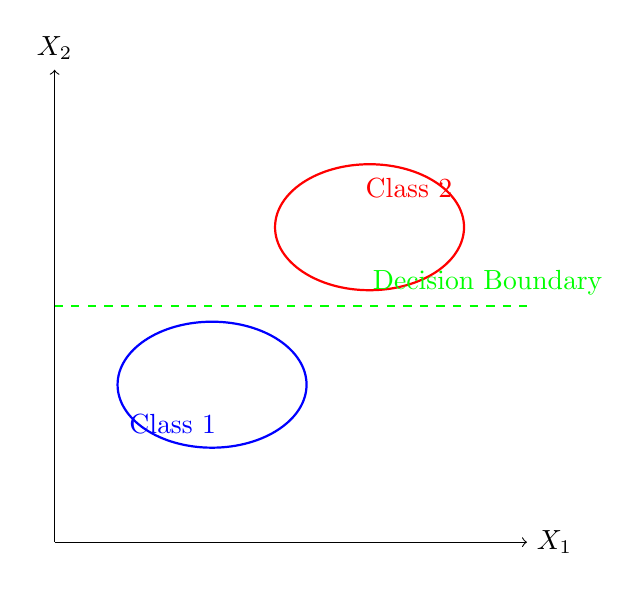
\begin{tikzpicture}[scale=1.0]
% axes
\draw[->] (0,0) -- (6,0) node[right] {$X_1$};
\draw[->] (0,0) -- (0,6) node[above] {$X_2$};

% class 1 ellipse
\draw[blue, thick] (2,2) ellipse (1.2cm and 0.8cm);
\node[blue] at (1.5,1.5) {Class 1};

% class 2 ellipse
\draw[red, thick] (4,4) ellipse (1.2cm and 0.8cm);
\node[red] at (4.5,4.5) {Class 2};

% linear decision boundary
\draw[green, thick, dashed] (0,3) -- (6,3);
\node[green] at (5.5,3.3) {Decision Boundary};
\end{tikzpicture}

\subsubsection{Quadratic Discriminant Analysis (QDA)}

QDA relaxes the LDA assumption of common covariance matrices:
\[
\Sigma_k \neq \Sigma_j \quad \text{for some } k \neq j
\]

The discriminant function becomes quadratic:
\[
\delta_k(x) = -\frac{1}{2} \log |\Sigma_k| - \frac{1}{2} (x - \mu_k)^T \Sigma_k^{-1} (x - \mu_k) + \log \pi_k
\]

\subsubsection{Naive Bayes Classifier}

Naive Bayes assumes that features are conditionally independent given the class:
\[
P(X_1, X_2, \dots, X_p \mid Y=k) = \prod_{j=1}^p P(X_j \mid Y=k)
\]

This allows simple estimation using Gaussian distributions for quantitative features or categorical probabilities for discrete features.

\subsubsection{K-Nearest Neighbors (KNN)}

\begin{itemize}
    \item Non-parametric and flexible
    \item Assigns a class based on the majority vote of the \(K\) nearest neighbors in feature space
    \item More data generally improves performance
\end{itemize}

\subsubsection{Bias-Variance Trade-off and Model Comparison}

\begin{itemize}
    \item LDA: Linear boundaries, low variance, higher bias
    \item QDA: Quadratic boundaries, higher variance, lower bias
    \item Logistic Regression: Linear boundary, sensitive to collinearity
    \item KNN: Highly flexible, low bias, potentially high variance
\end{itemize}

\subsubsection{Performance Metrics}

\begin{itemize}
    \item \textbf{Accuracy:} Overall correct classification
    \item \textbf{Sensitivity / Recall:} True positive rate
    \item \textbf{Specificity:} True negative rate
    \item \textbf{ROC curve:} Trade-off between sensitivity and false positive rate
\end{itemize}

\subsubsection{Other Notes}

\begin{itemize}
    \item Poisson regression for count data: \(n \sim \text{Poisson}(\mu)\) with \(\log(\mu) = X \beta\)
    \item More data allows more flexible models (e.g., QDA, KNN) to perform well without overfitting
\end{itemize}
